\chapter{Fundamentals}
\label{cha:Chapter3_Fundamentals}
\iffalse

Length: eher 10 pages, kann auch weniger sein

Effort: ~3-4 weeks

Hier auch mehr zu Data Mining --> fundamental
Allgemeine Techniken eher knapp, je spezifischer desto detaillierter in meine Richtung
Nur Themen, die nicht originaer von mir kommen
Muss nicht jedem erklaerbar sein --> Basislevel voraussetzen
Viele Referenzen bringen, Zitate

Questions:
\begin{itemize}
\item TODO
\end{itemize}

Content
\begin{itemize}
\item Data Mining
\item Sentiment Analysis
\begin{itemize}
\item Definition/Overview
\item Approaches
\begin{itemize}
\item Lexicon-Based
\item Machine Learning \begin{itemize}
    \item Unigram vs. n-gram/bi-gram
    \item Stop words?
    \item 
\end{itemize}
\item Hybrid
\end{itemize}
\end{itemize}
\item Twitter
\begin{itemize}
\item Overview, gehoert auch dazu, etwas knapper
\item Challenges
\end{itemize}
\end{itemize}
\fi


\section{Twitter}
Twitter is a microblogging service, which allows users to send messages, so-called "tweets", containing text, media, or links. It is one of the largest social media platforms, with 330 Million monthly users in the first quartal of 2019 posting 500 million messages daily \cite{twitter:users}. It was launched in 2006 and differentiates itself from other platforms by the focus on short messages. The length of a tweet was originally restricted to 140 characters, until the company expanded the size to 280 characters in 2017 \cite{twitter:characters}. Due to this, Twitter offers a large number of short messages on varying topics made by varying user groups. 
\TODO{tweet id}

Figure \ref{fig:example_tweet} shows an example of a tweet, in this case, a tweet by NASA for the Phoenix mission. An account is identified by its unique username, in the example tweet "@MarsPhoenix". There are several ways to interact with a tweet. First, a tweet can be responded to. Next, a tweet can be retweeted, which shares the tweet to a user's profile, or quoted, which adds a comment to the retweet. Finally, a tweet can be liked. Other users can also be mentioned in a tweet, with their username being identified by the "@" symbol. 

\begin{figure}
    \centering
    
\includegraphics[scale=0.3]{Images/twitter_image.png}
    \caption{Picture of a tweet made by the @MarsPhoenix account. \TODO{english}}
    \label{fig:example_tweet}
\end{figure}

Several of Twitter's characteristics can be further examined.
First, the short length. Bermingham and Smeaton compared the classification of sentiment on microblogs with longer documents and concluded that it is easier to classify microblogs \cite{microblogs}.

Furthermore, informal usage of English and length restrictions frequently lead to abbreviations, slang, and misspellings, which must be considered during feature selection. This leads to data sparsity, as many terms appear infrequently over an entire corpus. Saif et al. observed that "93\% of the words in the tweet data occur less than 10 times" \cite[p.~3]{data_sparsity}, compared to 78\% in movie review data. Hashtags are often used to assign a tweet to a certain topic by writing "\#topic". The topics itself deal with a large variety of topics, such as politics, sports, and music.

Twitter offers two APIs (application programming interface) to retrieve and analyze Twitter data, REST and Streaming \cite{DBLP:journals/csur/GiachanouC16}. There currently are three different access levels, which provide different rates and limit. The Elevated level, for example, allows the retrieval of up to 2 million tweets per month \cite{twitter:about}. Using the REST API, several functionalities can be accessed, such as the lookup of tweets, users, the creation and deletion fo tweets and much more. Generally speaking, the REST API provides a short-lived connection. Most importantly, the REST API can be used to search for tweets. Twitter differentiates between recent search, which provides access to public Tweets posted in the last week, and full-archive search, which makes every Tweet made since the first one in 2006 available. For full-archive search, academic research access is needed. Tweets can be filtered according to parameters such as language, content, and type (e.g. retweet) \cite{twitter:search}. 

The streaming API, on the other hand, allows developers to access a real-time stream of Tweets, which can be filtered according to rules \cite{twitter:stream}. All information is returned in a JSON format, which can be easily parsed by many programming languages. Thus, the Twitter API provides a great method to collect large amounts of tweets \cite{DBLP:journals/csur/GiachanouC16}.


\section{Data Mining}
Because of the massive amount of data that is collected every day, processing and extracting information becomes more valuable and challenging. Tan et al. describe Data Mining as "[blending] traditional data analysis methods with sophisticated algorithms to process this abundance of data" \cite[p.~21]{DBLP:books/aw/TanSKK2019}. Data Mining faces a few challenges. First, scalability is important, as the amount of data that can be collected and stored is constantly growing. Next, dimensionality has to be considered, which describes the number of attributes a data set has. If, for example, multiple measurements of the same data point need to be taken into account, each measurement becomes an attribute. Furthermore, the types of data are becoming more complex, as data from fields such as social media, DNA research, and climate are analyzed \cite{DBLP:books/aw/TanSKK2019}.

Data Mining can be separated into two different groups. Predictive tasks try to predict an attribute value, the target variable, using other attribute values, also called explanatory variables. Descriptive tasks identify patterns, such as correlation, to understand relationships in data. Predictive modeling, according to Tan et al., "refers to the task of building a model for the target variable as a function of the explanatory variable" \cite[p.~29]{DBLP:books/aw/TanSKK2019}. This can be divided into classification for discrete target variables and regression for continuous target variables. In this thesis, classification is used, which is illustrated in Figure \ref{fig:classifiation}. A collection of instances is used, which are defined by the tuple $(x,y)$, with $x$ being a set of attribute values, and $y$ being the class label, which must be categorical. The classification model describes the relationship between the attribute set $x$ and the class label $y$ and can be expressed as a function $f$, which takes in the attribute set $x$ and returns a class label. If $f(x) = y$ for an instance $(x,y)$, the instance is correctly classified.
\begin{figure}
    \centering
    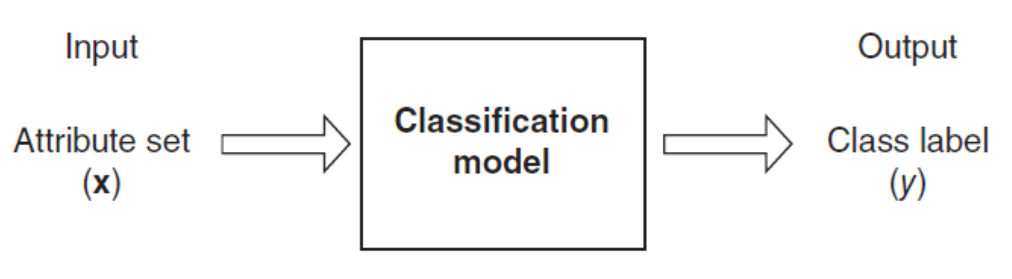
\includegraphics[scale = 0.6]{Images/classification.png}
    \caption{A schematic illustration of a classification task by Tan et al. \cite[p.~134]{DBLP:books/aw/TanSKK2019}.}
    \label{fig:classifiation}
\end{figure}


%\TODO{maybe difference opinion, sentiment, subjectivity?}
%According to Pang and Lee Sentiment Analysis "deals with the computational treatment of [...] opinion, sentiment, and subjectivity in text" \cite[p.~5]{DBLP:journals/ftir/PangL07}.  Pang and Lee suggest several applications for Sentiment Analysis, such as review-related websites, in addition to existing technologies such as recommendation systems, as well as business and government intelligence \cite[p.~8]{DBLP:journals/ftir/PangL07}.

\section{Sentiment Analysis}
Liu defines sentiment analysis, also known as opinion mining, as "the field of study that analyzes people's opinions, sentiments, appraisals, attitudes, and emotions toward entities and their attributes expressed in written text" \cite[p.~1]{liu_2015}. He states that entities include "products, services, organizations, individuals, events, issues, or topics" \cite[p.~1]{liu_2015}. He further analyzes the difference between sentiment and opinion, citing the Merriam-Webster dictionary. There, "sentiment is defined as an attitude, thought, or judgment prompted by feeling, while opinion is defined as a view, judgment, or appraisal formed in the mind" \cite[p.~2]{liu_2015}. Through this definition, a subtle difference can be seen, where sentiment tends to be viewed more as a feeling, while an opinion is a more concrete view. While this difference exists, Sentiment Analysis and Opinion Mining are still used interchangeably to refer to the same field. Liu defines the term opinion as an encompassing term that includes not only sentiment, but also additional information, such as the opinion holder. A more formal definition for an opinion by Liu, can be seen in Equation \eqref{eq:opinion}:
\begin{equation}
    opinion = (e, a, s, h, t),
    \label{eq:opinion}
\end{equation}
where $e$ denotes an entity, $a$ is an aspect of $e$ that is targeted, $s$ is the sentiment, $h$ describes the opinion holder, and $t$ the time when the opinion was published \cite{liu_2015}. To further illustrate the difference, the example sentence "I like the display of my iPad." published on 07.05.2022 by Max Mustermann is considered. Here, the entity $e$ is the target of the opinion, the iPad, while $a$ is the specific attribute of the iPad that the sentiment is based on, in this case, the display. Finally, the sentiment $s$ is qualified as positive, the opinion holder $h$ is Max Mustermann, and the time $t$ is 07.05.2022, resulting in the quintuple (iPad, Display, Positive, Max Mustermann, 07.05.2022). If an opinion does not target a specific aspect, but rather the entire entity, the aspect is defined as "GENERAL" \cite{liu_2015}. 


Liu identified three different levels of analysis. The document level classifies an entire document as positive or negative, while assuming that it relates to a single entity, such as in a product review. The next level is the sentence level, which determines the sentiment of each sentence, including neutral if the sentence does not contain an opinion. The aspect level includes the entity and aspect with which an opinion is concerned \cite{liu_2015}.

Most research differentiates between two tasks in Sentiment Analysis. Pang and Lee, for example, differentiate between detection of polarity and detection of subjectivity. The most common form of polarity detection is called sentiment polarity classification, which aims to label an opinionated document as either positive or negative. Polarity may also be viewed as a multi-class problem, where the degrees of positivity are considered, as well as the neutral class, which Pang and Lee describe as the middle ground between positive and negative. Subjectivity detection, on the other hand, seeks to determine whether a given text contains a subjective opinion or is objective. Pang and Lee note that they make a distinction between neutral and objective, the latter being a lack of opinion \cite{DBLP:journals/ftir/PangL07}. Other researchers such as Liu define neutral as being the lack of opinion, noting that an objective sentence may still imply sentiment \cite{liu_2015}. Especially in human-coded data sets, the difference between objective and neutral is often a problem. Nakov et al. instructed their coders to determine whether a sentence is objective, positive, negative, or neutral. For their sentence polarity task, they combined sentences with an objective and neutral score to one class, as the coders often mixed the two classes \cite{nakov-etal-2013-semeval}.

\begin{figure}
    \centering
    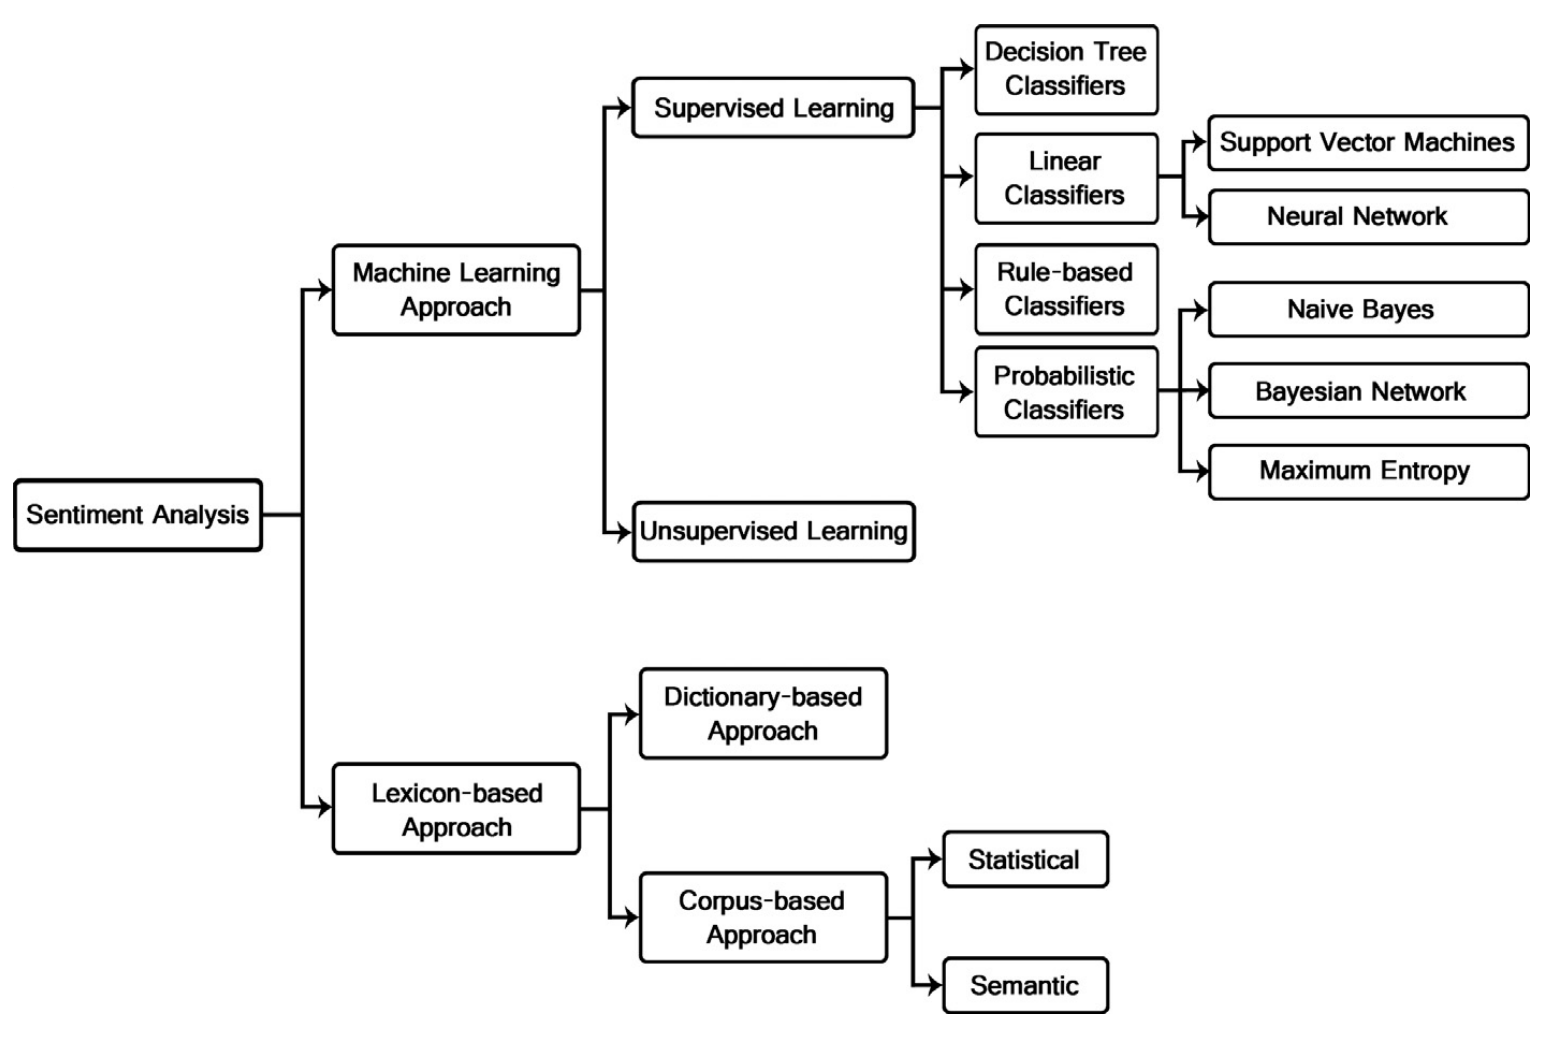
\includegraphics[scale=0.3]{Images/classification_techniques.png}
    \caption{Sentiment classification techniques by Medhat et al. \cite{MEDHAT20141093}}
    \label{fig:classifiers}
\end{figure}


For polarity classification, Medhat et al. divide techniques into three categories, machine learning, lexicon-based, and hybrid \cite{MEDHAT20141093}. They show the most important classifiers in Figure \ref{fig:classifiers}. In general, the machine learning approach treats Sentiment Analysis as a text classification problem using training data to classify unknown instances. Supervised machine learning uses labeled training documents together with classifiers such as Naive Bayes. Because it can be difficult to generate a large number of labeled training data, unsupervised approaches are also used, which rely solely on unlabeled data \cite{MEDHAT20141093}. The supervised methods are further subdivided. According to Tan et al., probabilistic classifiers, such as Naive Bayes and Logistic Regression, "make use of probability theory to represent the relationship between attributes and class labels" \cite[p.~414]{DBLP:books/aw/TanSKK2019}. Linear classifiers, on the other hand, try to find a hyperplane to separate instances from different classes \cite{MEDHAT20141093}. Decision Tree Classifiers, for example, Random Forest, use attribute values to divide the data into a tree structure. In Sentiment Analysis, the presence/frequency of words is often used for decisions. Finally, rule-based classifiers utilize a set of rules to classify an instance \cite{DBLP:books/aw/TanSKK2019}.

The lexicon-based approach makes use of a sentiment lexicon, which contains sentiment words and their values. In addition, intensifiers and negations may be used. To classify a document, all the values of sentiment words detected in the document are summed up, if the sum is positive the document is classified as negative, if the sum is 0 as neutral, and if the sum is negative as negative. By using negations and intensifiers, the sentiment values are adjusted \cite{liu_2015}. There are three different approaches to building a sentiment lexicon, which are outlined by Medhat et al. There is the manual collection of words, which is, of course, very time-intensive. Next, a dictionary-based approach can be used. This method starts with a small list of opinion words, and then searches dictionaries such as WordNet for synonyms and antonyms, maintaining the orientations for synonyms and reversing them for antonyms. The found words are then added to the list and used for the next iteration. The corpus-based approach utilizes context-specific orientations along with a list of opinion words to find opinion words in a large corpus. It is based on sentiment consistency, which assumes that adjective conjoined by e.g. "and" have the same polarity, while "but" would signify opposing polarities. This approach can be further subdivided into statistical approaches, which finds co-occurrence patterns using statistics, and semantic approaches, which utilizes semantic relationships \cite{MEDHAT20141093}.







